% -*- root: main.tex -*-

\chapter{Unoriented bordism}\label{UnorientedBordismChapter}


\todo{Write an introduction for me.}


\section{Thom spectra and the Thom isomorphism}\label{LectureThomSpectra}

Our first case study is a sequence of theorems about the unoriented bordism spectrum $MO$.  I wanted to begin by recalling one definition of the spectrum $MO$, since it involves ideas that will be useful to us throughout the semester.

\begin{definition}
For a spherical bundle $S^{n-1} \to \xi \to X$, its Thom space is given by the cofiber \[\xi \to X \xrightarrow{\text{cofiber}} T(\xi).\]
\end{definition}
\begin{proof}[``Proof'' of definition]
There is a more classical construction of the Thom space: take the associated disk bundle by gluing an $n$--disk fiberwise, and add a point at infinity: \[T(\xi) = (\xi \sqcup'_{S^{n-1}} D^n)^+.\]  To compare this with the cofiber definition, recall that the thickening of $\xi$ to an $n$--disk bundle is the same thing as taking the mapping cylinder on $\xi \to X$.  Since the inclusion into the mapping cylinder is now a cofibration, the quotient by this subspace agrees with both the cofiber of the map and the introduction of a point at infinity.
\end{proof}

Before proceeding, here are two important examples:
\begin{example}\label{TrivialBundleThomExample}
If $\xi = S^{n-1} \times X$ is the trivial bundle, then $T(\xi) = S^n \sm (X_+)$.  This is supposed to indicate what Thom spaces are ``doing'': if you feed in the trivial bundle then you get the suspension out, so if you feed in a twisted bundle you should think of it as a \textit{twisted suspension}.
\end{example}

\begin{example}\label{RPnThomExample}
Let $\xi$ be the tautological $S^0$--bundle over $\RP^\infty = BO(1)$.  Because $\xi$ has contractible total space, $EO(1)$, the cofiber degenerates and it follows that $T(\xi) = \RP^\infty$. More generally, arguing by cells shows that the Thom space for the tautological bundle over $\RP^n$ is $\RP^{n+1}$.
\end{example}

\todo{Two people (Mauro and someone else) asked in what generality this ``$Bh\Aut F$'' construction works.  This can be clarified in a remark.}
Now we catalog a bunch of useful properties of the Thom space functor. Firstly, recall that a spherical bundle over $X$ is the same data as a map $X \to B \GL_1 S^{n-1}$, where $\GL_1 S^{n-1}$ is the subspace of $F(S^{n-1}, S^{n-1})$ expressed by the pullback\todo{In lecture, you decided to call these $B h\operatorname{Aut}(S^{n-1})$, which is maybe a healthier choice?} \todo{does this mean we are regarding $h\operatorname{Aut}(S^{n-1})$ as a group? Is $\operatorname{Aut}(S^{n-1})$ a topological group? Would it make sense to say $B \operatorname{Aut}(S^{n-1})$? To be honest I personally like $GL_1S^n$. It might cause some potential for confusion but it looks more clean. - danny}
\begin{center}
\begin{tikzcd}
\GL_1 S^{n-1} \arrow{r} \arrow{d} & F(S^{n-1}, S^{n-1}) \arrow{d} \\
\Aut_{h\CatOf{Spaces}} S^{n-1} \arrow{r} & \End_{h\CatOf{Spaces}} S^{n-1} \arrow[-,double]{r} & \pi_0 F(S^{n-1}, S^{n-1}).
\end{tikzcd}
\end{center}
We can interpret $T$ as a functor off of the slice category over $BGL_1 S^{n-1}$: maps \[Y \xrightarrow{f} X \xrightarrow{\xi} B \GL_1 S^{n-1}\] induce maps $T(f^* \xi) \to T(\xi)$, and $T$ is suitably homotopy-invariant.

\todo{You can make this section clearer by noticing that the map $J_{\R}^n$ is directly induced by a map $O(n) \to h\Aut S^{n-1}$ by the action of $O(n)$ on $\R^n$.  This makes the commutativity of the relevant diagrams clear, whereas using the Yoneda lemma does not make it clear that we can take the appropriate homotopy colimits.  --Mauro}
Next, the spherical subbundle of a vector bundle gives a common source of spherical bundles.  Since rank $n$ vector bundles are also classified by an object $BO(n)$, this begets a map $J_{\R}^n\co BO(n) \to B \GL_1 S^{n-1}$ for each $n$.  Stable homotopy theorists are very interested in the block--inclusion maps $i^n\co BO(n) \to BO(n+1)$ and the colimit $BO = BO(\infty)$.  The suspension functor induces a map $\GL_1 S^{n-1} \to \GL_1 S^n$, and we are led to ask about the compatibility of these operations.  As a route to answering this, the block--inclusion maps are a special case of a more general direct sum map $\oplus\co BO(n) \times BO(m) \to BO(n+m)$, given by the precomposition \[BO(n) = BO(n) \times * \xrightarrow{\operatorname{id} \times \text{triv}} BO(n) \times BO(1) \xrightarrow\oplus BO(n+1).\] The spaces $B \GL_1 S^{n-1}$ enjoy a similar ``collective monoid'' structure, given by taking the fiberwise join two spherical bundles with a common base.
\begin{lemma}
The fiberwise join is represented by maps \[B\GL_1 S^{n-1} \times B\GL_1 S^{m-1} \to B\GL_1 S^{n+m-1},\] and these maps commute with the block sum maps on the $BO(n)$ family: \todo{Split the left vertical arrow into two?} \todo{Index it by $J_\mathbb{R}^n \times J_\mathbb{R}^m$, and the right vertical arrow by $J_\mathbb{R}^{n+m}$? -Danny}
\begin{center}
\begin{tikzcd}
BO(n) \times BO(m) \arrow{d} \arrow{r} & BO(n+m) \arrow{d} \\
B\GL_1 S^{n-1} \times B\GL_1 S^{m-1} \arrow{r} & B\GL_1 S^{n+m-1}.
\qed
\end{tikzcd}
\end{center}
\end{lemma}
\noindent Again taking a cue from $K$--theory, we take the colimit as $n$ grows large.
\begin{corollary}
There is a map of $H$--spaces $J_{\R}\co BO \to B\GL_1 \S$ called the \textit{stable $J$--homomorphism}. \qed
\end{corollary}
\noindent Finally, we can ask about the compatibility of $T$ with all of this:\todo{The right place to address dimension is here.  $T$, as defined above, does not extend to a functor off of the system $\{BhAut(S^{n-1})\}$ unless you reduce each Thom complex by the appropriate dimension shift.}
\begin{lemma}\label{ThomSpacesAreMonoidal}
$T$ is monoidal: it carries external fiberwise joins to smash products of Thom spaces. \qed
\end{lemma}

We are now prepared to define our spectrum $MO$.  The unstable $J$--maps $J_{\R}^n\co BO(n) \to B\GL_1 S^{n-1}$ give Thom spaces $T(J_{\R}^n)$,\todo{Be careful about dimension here: you really mean a reduced tautological bundle, related to how $BO$ has only one connected component.} equipped with maps\todo{Fix this equation.}\todo{What's wrong with it?-danny} \[\Susp T(J_{\R}^n) = T(J_{\R}^n \oplus \text{triv}) \to T(J_{\R}^{n+1}).\] Setting $MO(n) = \Susp^{-n} \Susp^\infty T(J_{\R}^n)$, we again assemble this data into a single object: \[MO := \colim_n MO(n) = \colim_n \Susp^{-n} T(J_{\R}^n).\]
\todo{Question: You essentially defined $MO$ here by piecing together the $T(J_\mathbb{R}^n)$'s. We should mention that another way to pack all this info together is to say $MO = T(J_\mathbb{R})$ -danny}
\todo{There should be a Theorem here saying that we recover $MO$ as defined on the first day.}

The spectrum $MO$ has several remarkable properties.  The most basic such property is that it is a ring spectrum, and this follows immediately from $J_{\R}$ being a homomorphism of $H$--spaces.  Much more excitingly, we can also deduce the presence of Thom isomorphisms just from the properties stated thus far.  That $J_{\R}$ is a homomorphism means that the following square commutes:
\begin{center}
\begin{tikzcd}
BO \times BO \arrow{r}{\sigma, \simeq} \arrow[bend right]{rrd} & BO \times BO \arrow{r}{\mu} \arrow{d}{J_{\R} \times J_{\R}} & BO \arrow{d}{J_{\R}} \\
& B\GL_1 \S \times B\GL_1 \S \arrow{r}{\mu} & B\GL_1 \S.
\end{tikzcd}
\end{center}
We have extended this square very slightly by a certain shearing map $\sigma$ defined by $\sigma(x, y) = (xy^{-1}, y)$.\todo{$\sigma$ \emph{almost} shows up in giving a categorical definition of a $G$--torsor.  I wish I understood this, but I always get tangled up.}  It's evident that $\sigma$ is a homotopy equivalence, since just as we can de-scale the first coordinate by $y$ we can re-scale by it.  We can calculate directly the behavior of the long composite: \[J_{\R} \circ \mu \circ \sigma(x, y) = J_{\R} \circ \mu(xy^{-1}, y) = J_{\R}(xy^{-1}y) = J_{\R}(x).\]  It follows that the second coordinate plays no role, and that the bundle classified by the long composite can be written as $J_{\R} \times 0$.\footnote{This factorization does \emph{not} commute with the rest of the diagram, just with the little triangle it forms.} \todo{I'm confused about the commutativity of this factorization with the rest of the diagram.-danny}  We are now in a position to see the Thom isomorphism:
\begin{lemma}[Thom isomorphism, universal example] As $MO$--modules,\todo{Is it clear that this is an equivalence of $MO$--modules? This should come from the $x$--factor being unmolested, right?}\todo{Is it furthermore clear that the cohomological version of this gives an action of $E^* X$ on $E^* T(\xi)$ by the ``Thom diagonal''?} \[MO \sm MO \simeq MO \sm \Susp^\infty_+ BO.\]
\end{lemma}
\begin{proof}
Stringing together the naturality properties of the Thom functor outlined above, we can thus make the following calculation:
\begin{align*}
T(\mu \circ (J_{\R} \times J_{\R})) & \simeq T(\mu \circ (J_{\R} \times J_{\R}) \circ \sigma) & \text{(homotopy invariance)} \\
& \simeq T(\mu \circ (J_{\R} \times 0)) & \text{(constructed lift)} \\
& \simeq T(J_{\R}) \sm T(0) & \text{(monoidality)} \\
& \simeq T(J_{\R}) \sm \Susp^\infty_+ BO & \text{(\Cref{TrivialBundleThomExample})} \\
T(J_{\R}) \sm T(J_{\R}) & \simeq T(J_{\R}) \sm \Susp^\infty_+ BO & \text{(monoidality)} \\
MO \sm MO & \simeq MO \sm \Susp^\infty_+ BO. & \text{(definition of $MO$)} & \phantom{.} \qedhere
\end{align*}
\end{proof}

\noindent From here, the general version of Thom's theorem follows quickly:

\begin{theorem}[Thom isomorphism]
Let $\xi\co X \to BO$ classify a vector bundle and let $\phi: MO \to E$ be a map of ring spectra. Then there is an equivalence of $E$--modules \[E \sm T(\xi) \simeq E \sm \Susp^\infty_+ X.\]
\end{theorem}
\begin{proof}[Modifications to above proof]
To accommodate $X$ rather than $BO$ as the base, we redefine $\sigma\co BO \times X \to BO \times X$ by \[\sigma(x, y) = \sigma(x \xi(y)^{-1}, y).\]  This gives an equivalence $MO \sm T(\xi) \simeq MO \sm \Susp^\infty_+ X$.  To introduce $E$, note that there is a diagram
\begin{center}
\begin{tikzcd}
E \sm T(\xi) \arrow[densely dotted]{r}{\simeq} \arrow{d}{\eta_{MO} \sm \id \sm \id} & E \sm \Susp^\infty_+ X \arrow{d}{\eta_{MO} \sm \id \sm \id} \\
MO \sm E \sm T(\xi) \arrow{r}{\simeq} \arrow{d}{(\mu \circ (\phi \sm \id)) \sm \id} & MO \sm E \sm \Susp^\infty_+ X \arrow{d}{(\mu \circ (\phi \sm \id)) \sm \id} \\
E \sm T(\xi) \arrow{r} & E \sm \Susp^\infty_+ X.
\end{tikzcd}
\end{center}
The middle equivalence comes from the previous Thom isomorphism, smashed through with $E$.  The bottom arrow exists by applying the action map to both sides.  Reusing the bottom arrow at the top arrow and using the unitality of the monoid $E$ shows the map to be an equivalence. \todo{I'm a little confused here. Once we have the equivalence $MO \wedge T(\xi) \simeq MO \wedge \Sigma_+^\infty X$, why can't be apply $(\varphi, id)$ to this equivalence to obtain $E \wedge T(\xi) \simeq E \wedge \Sigma_+^\infty X$? -danny}
\end{proof}
\todo{At least hint that there's a converse to this Theorem, to be explored later.}

\begin{example}
We'll close out today by using this to actually make a calculation. Recall from \Cref{RPnThomExample} that $T(\L - 1 \downarrow \RP^n) = \RP^{n+1}$.\todo{Is there a disuspension here?-danny}  By killing all the homotopy elements in positive degrees, we can also see that the map $MO \to H\F_2$ is a ring map\todo{This requires some justification, like $MO$ being connective .}, so that we can apply the Thom isomorphism theorem to the mod--$2$ homology of Thom complexes coming from real vector bundles:
\begin{align*}
\pi_* (H\F_2 \sm T(\L - 1)) & \cong \pi_* (H\F_2 \sm T(0)) & \text{(Thom isomorphism)} \\
\pi_* (H\F_2 \sm \Susp^{-1} \Susp^\infty \RP^{n+1}) & \cong \pi_* (H\F_2 \sm \Susp^\infty_+ \RP^n) & \text{(\Cref{RPnThomExample})} \\
\widetilde{H\F_2}_{*+1} \RP^{n+1} & \cong H\F_2{}_* \RP^n. & \text{(generalized homology)}
\end{align*}
This powers an induction that shows $H\F_2{}_* \RP^\infty$ has a single class in every degree.  \todo{Wouldn't hurt to expand on this.}  The cohomology version of all this, together with the $H\F_2^* \RP^n$--module structure of $H\F_2^* T(\L-1)$, also gives the ring structure: \[H\F_2^* \RP^n = \F_2[x] / x^{n+1}.\] \todo{This part is interesting. I just remembered that the Thom isomorphism theorem I know is actually about cohomology! What's the similar story for cohomology here? We should talk about this. -danny}
\end{example}






\section{Cohomology rings and affine schemes}

\todo[inline]{Make sure you use $\F_2$ everywhere, rather than $\Z/2$.}
An abbreviated summary of this semester is that we're going to put ``$\Spec$'' in front of rings appearing in algebraic topology and see what happens.  Before doing any algebraic topology, let me remind you what this means on the level of algebra.  The core idea is to replace a ring $R$ by the functor it corepresents, $\Spec R$.  For any ``test $\F_2$--algebra'' $T$, we set \[(\Spec R)(T) := \CatOf{Algebras}_{\F_2/}(R, T) \cong \CatOf{Schemes}_{/\F_2}(\Spec T, \Spec R).\]  More generally, we have the following definition:
\begin{definition}
An \textit{affine $\F_2$--scheme} is a functor $X: \CatOf{Algebras}_{\F_2/} \to \CatOf{Sets}$ which is (noncanonically) isomorphic to $\Spec R$ for some $\F_2$--algebra $R$.  Given such an isomorphism, we will refer to $\Spec R \to X$ as a \textit{parameter} for $X$ and its inverse $X \to \Spec R$ as a \textit{coordinate} for $X$.
\end{definition}

\begin{lemma}
There is an equivalence of categories \[\Spec: \CatOf{Algebras}_{\F_2/}^{\mathrm{op}} \to \CatOf{AffineSchemes}_{/\F_2}. \qed\]
\end{lemma}

The centerpiece of thinking about rings in this way, for us and for now, is to translate between a presentation of $R$ as a quotient of a free algebra and a presentation of $(\Spec R)(T)$ as selecting tuples of elements in $T$ subject to certain conditions.  Consider the following example:
\begin{example}\label{FiniteOrderAffineSpaceDefn}
Set $R_1 = \F_2[x]$.  Then \[(\Spec R_1)(T) = \CatOf{Algebras}_{\F_2/}(\F_2[x], T)\] is determined by where $x$ is sent --- i.e., this Hom--set is naturally isomorphic to $T$ itself.  Consider also what happens when we impose a relation by passing to $R_2 = \F_2[x] / (x^{n+1})$.  The value \[(\Spec R_2)(T) = \CatOf{Algebras}_{\F_2/}(\F_2[x] / (x^{n+1}), T)\] of the associated affine scheme is again determined by where $x$ is sent, but now $x$ can only be sent to elements which are nilpotent of order $n+1$.  These schemes are both important enough that we give them special names:
\begin{align*}
\mathbb A^1 & := \Spec \F_2[x], & \mathbb A^{1, (n)} & := \Spec \F_2[x] / (x^{n+1}).
\end{align*}
The symbol ``$\mathbb A^1$'' is pronounced ``the affine line'' --- reasonable, since the value $\mathbb A^1(T)$ is, indeed, a single $T$'s worth of points.  Note that the quotient map $R_1 \to R_2$ induces an inclusion $\mathbb A^{1, (n)} \to \mathbb A^1$ and that $\mathbb A^{1, (0)}$ is a constant functor: \[\mathbb A^{1, (0)}(T) = \{f: \F_2[x] \to T \mid f(x) = 0\}.\]  Accordingly, we pronounce ``$\mathbb A^{1, (0)}$'' as ``the origin on the affine line'' and ``$\mathbb A^{1, (n)}$'' as ``the $n${\th} order (nilpotent) neighborhood of the origin in the affine line''\todo{except it is actually of order $n+1$. Mmm...}.
\end{example}

We can also express in this language another common object arising from algebraic topology: the Hopf algebra, which appears when taking the mod--$2$ cohomology of an $H$--group.  In addition to the usual cohomology, the extra pieces of data are those induced by the $H$--group multiplication, unit, and inversion maps, which on cohomology beget a diagonal map $\Delta$, an augmentation map $\eps$, and an antipode $\chi$ respectively.  Running through the axioms, one quickly checks the following:
\begin{lemma}
For a Hopf $\F_2$--algebra $R$, the functor $\Spec R$ is naturally valued in groups.  Such functors are called \textit{group schemes}.  Conversely, a choice of group structure on $\Spec R$ endows $R$ with the structure of a Hopf algebra.
\end{lemma}
\begin{proof}
The functor $\Spec \colon \CatOf{Algebras}_{\F_2 /}^{\mathrm{op}} \to \mathrm{Funct}(\CatOf{Algebras}_{\F_2 /}, \CatOf{Sets})$ takes limits into limits.
Since tensor products of $\F_2$-algebras compute pushouts in $\CatOf{Algebras}_{\F_2 /}$, we see that Hopf algebras are simply cogroup objects in $\CatOf{Algebras}_{\F_2 /}$.
These remarks imply that $\Spec$ takes Hopf algebras into group objects in $\mathrm{Funct}(\CatOf{Algebras}_{\F_2 /}, \CatOf{Sets})$.
Now, for any small category $\cal{C}$, one has
\[ \mathrm{Grp}( \mathrm{Funct}(\cal{C}, \CatOf{Sets}) ) \simeq \mathrm{Funct}(\cal{C}, \CatOf{Groups}). \]
The conclusion now follows from the fully faithfulness of $\Spec$.
\end{proof}

\begin{example}\label{InformalAdditiveGroupExample}
The functor $\mathbb A^1$ introduced above is naturally valued in groups: since $\mathbb A^1(T) \cong T$, we can use the addition on $T$ to make it into an abelian group.  When considering $\mathbb A^1$ with this group scheme structure, we notate it as $\mathbb G_a$.  Applying the Yoneda lemma, one deduces the following formulas for the Hopf algebra structure maps:
\begin{align*}
\mathbb G_a \times \mathbb G_a & \xrightarrow{\mu} \mathbb G_a & x_1 + x_2 & \mapsfrom x, \\
\mathbb G_a & \xrightarrow{\chi} \mathbb G_a & -x & \mapsfrom x, \\
\Spec \F_2 & \xrightarrow{\eta} \mathbb G_a & 0 & \mapsfrom x.
\end{align*}
\end{example}

\begin{remark}
In fact, $\mathbb A^1$ is naturally valued in \emph{rings}. It models the inverse functor to $\Spec$ in the equivalence of categories above, i.e., the elements of a ring $R$ always form a complete collection of $\A^1$--valued functions on some affine scheme $\Spec R$ \todo{We haven't defined $\A^1$ at this point yet -danny}.
\end{remark}

\begin{example}
We define the \textit{multiplicative group scheme} by\todo{Do you want this to be a $\Z$--algebra? Ditto with $\mathbb A^1$ and $\mathbb G_a$?} \[\mathbb G_m = \Spec \F_2[x, y] / (xy - 1).\]  Its value $\mathbb G_m(T)$ on a test algebra $T$ is the set of pairs $(x, y)$ such that $y$ is a multiplicative inverse to $x$, and hence $\mathbb G_m$ is valued in groups.  Applying the Yoneda lemma, we deduce the following formulas for the Hopf algebra structure maps:
\begin{align*}
\mathbb G_m \times \mathbb G_m & \xrightarrow{\mu} \mathbb G_m & x_1 \otimes x_2 & \mapsfrom x \\
& & y_1 \otimes y_2 & \mapsfrom y, \\
\mathbb G_m & \xrightarrow{\chi} \mathbb G_m & (y, x) & \mapsfrom (x, y), \\
\Spec R & \xrightarrow{\eta} \mathbb G_m & 1 & \mapsfrom x, y.
\end{align*}
\end{example}

\begin{remark}
As presented above, the multiplicative group comes with a natural inclusion $\mathbb G_m \to \mathbb A^2$.  Specifically, the subset $\mathbb G_m \subseteq \mathbb A^2$ consists of pairs $(x, y)$ in the graph of the hyperbola $y = 1/x$.  However, the element $x$ also gives an $\mathbb A^1$--valued function $x\co \mathbb G_m \to \mathbb A^1$, and because multiplicative inverses in a ring are unique, we see that this map too is an inclusion.  These two inclusions have rather different properties relative to their ambient spaces, and we'll think harder about these essential differences later on.
\end{remark}

\begin{example}
The following example shows that it is a bad idea to think of affine group schemes as a schemeified version of linear lie groups.  Define the group scheme $\alpha_2$ to be $\mathrm{Spec}(\mathbb{F}_2[x]/(x^2))$ with group scheme structure given by
\begin{align*}
\alpha_2 \times \alpha_2 &\xrightarrow{\mu} \alpha_2 & x_1 + x_2 \mapsfrom x, \\
\alpha_2 & \xrightarrow{\chi} \alpha_2 & -x & \mapsfrom x, \\
\Spec \F_2 & \xrightarrow{\eta} \alpha_2 & 0 & \mapsfrom x.
\end{align*}

This group scheme has several interesting properties:
\begin{enumerate}
\item $\alpha_2$ has the same underlying structure ring as $\mu_2 = \mathbb{G}_m[2]$ but is not isomorphic to it.  The easiest way to see this is that $\mathrm{Hom}(\mu_2, \mu_2) = \mathbb{Z}/2\mathbb{Z}$ but $\mathrm{Hom}(\alpha_2, \mu_2) = \alpha_2$ (these homs are in the category of affine group schemes and give out an affine group scheme).
\item There is no commutative group scheme $G$ of rank four such that $\alpha_2 = G[2]$.
\item If $E/\mathbb{F}_2$ is the supersingular elliptic curve, then there is a short exact sequence $0 \rightarrow \alpha_2 \rightarrow E[2] \rightarrow \alpha_2 \rightarrow 0$.  However, this short exact sequence doesn't split (even after making a base change).
\item The subgroups of $\alpha_2 \times \alpha_2$ of order two are parameterized by $\mathbb{P}^1$.  That is to say. if $R$ is an $\mathbb{F}_2$-algebra, then the subgroup schemes of $(\alpha_2 \times \alpha_2)_R$ of order two defined over $R$ are parameterized by $\mathbb{P}^1(R)$.
\end{enumerate}
\end{example}

Additionally, the colimit of the sets $\colim_{n \to \infty} \mathbb A^{1,(n)}(T)$ is of use in algebra: it is the collection of nilpotent elements in $T$.  These kinds of conditions which are ``unbounded in $n$'' appear frequently enough that we are moved to give these functors a name too:
\begin{definition}
An \textit{affine formal scheme} is an ind-system of finite affine schemes.  \todo{Several people had questions about the utility of this. Does it just add certain colimits to the category of \emph{finite} affine schemes?}  The morphisms between such schemes are computed by \[\CatOf{FormalSchemes}(\{X_\alpha\}, \{Y_\beta\}) = \lim_\beta \colim_\alpha \CatOf{Schemes}(X_\alpha, Y_\beta).\]\todo{Question: can we reverse the order of taking lim and colim here?-danny}
\end{definition}

\begin{example}\label{FormalGaExample}
The individual schemes $\mathbb A^{1, (n)}$ do not support group structures.  After all, the sum of two elements which are nilpotent of order $n$ can only be guaranteed to be nilpotent of order $2n$. \todo{There is a minor indexing problem here. The elements corresponding to $A^{1, (n)}$ are actually nilpotent of order $n+1$} It follows that the entire ind-system $\{\mathbb A^{1, (n)}\} =: \A^1$ supports a group structure, even though none of its constituent pieces do.  We call such an object a \textit{formal group scheme}, and this particular formal group scheme we denote by $\G_a$.
\end{example}

\begin{example}
Similarly, one can define the scheme $\Gm[n]$ of elements of unipotent order $n$: \[\Gm[n] = \Spec \frac{\F_2[x,y]}{(xy - 1, x^n - 1)} \subseteq \Gm.\]  These \emph{are} all group schemes, but there is a second filtration along the lines of the one considered above: \[\Gm^{(n)} = \Spec \frac{\F_2[x,y]}{(xy - 1, (x - 1)^n)}.\]  These schemes are only occasionally group schemes.  The reader is invited\todo{Never invite the reader to do anything.} to check that there is an isomorphism $\{\Gm[n]\} \cong \{\Gm^{(n)}\}$ of formal schemes over $\F_2$, and that the induced formal group scheme structure on the right-hand side cannot be written level-wise --- rather, it involves the entire ind-scheme.\todo{Someone was interested in the relationship of this to the punctured formal scheme $\F_p(\!(q)\!)$.}
\end{example}

Let's now consider the example that we closed with last time, where we calculated $H\F_2^*(\RP^n) = \F_2[x] / (x^{n+1})$.  Putting ``$\Spec$'' in front of this, we could reinterpret this calculation as \[\Spec H\F_2^*(\RP^n) \cong \mathbb A^{1, (n)}.\]  This is such a useful thing to do that we will give it a notation all of its own:

\begin{definition}
Let $X$ be a finite cell complex, so that $H\F_2^*(X)$ is a ring which is finite--dimensional as an $\F_2$--vector space.  We will write \[X_{H\F_2} = \Spec H\F_2^* X\] for the corresponding finite affine scheme.
\end{definition}

\begin{example}
Putting together the discussions from this time and last time, in the new notation we have calculated \[\RP^n_{H\F_2} \cong \mathbb A^{1, (n)}.\]
\end{example}

So far, this example just restates things we knew in a mildly different language.  Our driving goal for the remainder of today and for tomorrow is to incorporate as much information as we have about these cohomology rings $H\F_2^* (\RP^n)$ into this description, which will result in us giving a more ``precise'' name for this object.  Along the way, we will discover why $X$ had to be a \emph{finite} complex and how to think about more general $X$.  For now, though, let's content ourselves with investigating the Hopf algebra structure on $H\F_2^* \RP^\infty$.

\begin{example}\label{RPExampleFaulty}
Recall that $\RP^\infty$ is an $H$--space in two equivalent ways:
\begin{enumerate}
\item There is an identification $\RP^\infty \simeq K(\Z/2, 1)$, and the $H$--space structure is induced by the sum on cohomology.
\item There is an identification $\RP^\infty \simeq BO(1)$, and the $H$--space structure is induced by the tensor product of real line bundles.
\end{enumerate}
In either case, this induces a Hopf algebra diagonal \[H\F_2^* \RP^\infty \otimes H\F_2^* \RP^\infty \xleftarrow\Delta H\F_2^* \RP^\infty\] which we would like to analyze.  This map is determined by where it sends the class $x$, and because it must respect gradings it must be of the form $\Delta x = ax_1 + bx_2$ for some constants $a, b \in \F_2$.  Furthermore, because it belongs to a Hopf algebra structure, it must satisfy the unitality axiom
\begin{center}
\begin{tikzcd}
H\F_2^* \RP^\infty \arrow[leftarrow]{r}{\begin{array}{c} \epsilon \otimes \id \\ \id \otimes \epsilon \end{array}} \arrow[leftarrow, bend right]{rr}{\id} & H\F_2^* \RP^\infty \otimes H\F_2^* \RP^\infty \arrow[leftarrow]{r}{\Delta} & H\F_2^* \RP^\infty.
\end{tikzcd}
\end{center}
and hence it takes the form \[\Delta(x) = x_1 + x_2.\]  Noticing that this is exactly the diagonal map in \Cref{InformalAdditiveGroupExample}, we tentatively identify ``$\RP^\infty_{H\F_2}$'' with the additive group.  This is extremely suggestive but does not take into account the fact that $\RP^\infty$ is an infinite complex, so we haven't allowed ourselves to write ``$\RP^\infty_{H\F_2}$'' just yet.  In light of the above discussion, we have left a very particular point open: it's not clear if we should use the name ``$\mathbb G_a$'' or ``$\G_a$''.  We will straighten this out tomorrow.
\end{example}








\section{The Steenrod algebra}\label{TheSteenrodAlgebraSection}

We left off yesterday with an ominous finiteness condition in our definition of $X_{H\F_2}$, and we produced a pair of reasonable guesses as to what ``$\RP^\infty_{H\F_2}$'' could mean.  It will turn out that we can answer which of the two guesses is reasonable by rigidifying the target category somewhat.  Here are the extra structures we will work toward incorporating:
\begin{enumerate}
\item Cohomology rings are \emph{graded}, and maps of spaces respect this grading.
\item Cohomology rings receive an action of the Steenrod algebra, and maps of spaces respect this action.
\item Both of these are complicated further when taking the cohomology of an infinite complex.
\item \label{SkewCommutativeDeficiency} (Cohomology rings for more elaborate cohomology theories are only skew-commutative, but ``$\Spec$'' requires a commutative input.)
\end{enumerate}
Today we will fix all these deficiencies of $X_{H\F_2}$ except for \#\ref{SkewCommutativeDeficiency}, which doesn't matter with mod--$2$ coefficients but which will be something of a bugbear throughout the rest of the semester.

Let's begin by considering the grading on $H\F_2^* X$.  In algebraic geometry, the following standard construction is used to track gradings:

\begin{definition}[{\cite[Definition 2.95]{StricklandFSFG}}]\todo{Maybe ``$\Z$--filtering'' is more appropriate.}
A \textit{$\Z$--grading} on a ring $R$ is a system of additive subgroups $R_k$ of $R$ satisfying $R = \bigoplus_k R_k$, $1 \in R_0$, and $R_j R_k \subseteq R_{j+k}$.  Additionally, a map $f\co R \to S$ of graded rings is said to \textit{respect the grading} if $f(R_k) \subseteq S_k$.
\end{definition}

\begin{lemma}[{\cite[Proposition 2.96]{StricklandFSFG}}]\label{GradedAndGmEquivAgree}
A graded ring $R$ is equivalent data to an affine scheme $\Spec R$ with an action by $\mathbb G_m$.  Additionally, a map $R \to S$ is homogeneous exactly when the induced map $\Spec S \to \Spec R$ is $\mathbb G_m$--equivariant.
\end{lemma}
\begin{proof}
A $\mathbb G_m$--action on $\Spec R$ is equivalent data to a coaction map \[\alpha^*: R \to R \otimes \F_2[x^\pm].\]  Define $R_k$ to be those points in $r$ satisfying $\alpha^*(r) = r \otimes x^k$.  It is clear that we have $1 \in R_0$ and that $R_j R_k \subseteq R_{j+k}$.  To see that $R = \bigoplus_k R_k$, note that every tensor can be written as a sum of pure tensors.  Conversely, given a graded ring $R$, define the coaction map on $R_k$ by \[(r_k \in R_k) \mapsto x^k r_k\] and extend linearly.
\end{proof}

This notion from algebraic geometry is somewhat different from what we are used to in algebraic topology, as it is designed to deal with things like polynomial rings (where the difference of two polynomials can lie in lower degree), but in classical algebraic topology we only ever encounter sums of terms with homogeneous degree.  We can modify our perspectively very slightly to arrive at the algebraic geometers': replace $H\F_2$ by the periodified spectrum \[H\F_2P = \bigvee_{j=-\infty}^\infty \Susp^j H\F_2.\]  This spectrum has the property that $H\F_2P^0(X)$ is isomorphic to $H\F_2^*(X)$ as ungraded rings, but now we can make sense of the sum of two classes which used to live in different $H\F_2$--degrees.  At this point we can manually craft the desired coaction map $\alpha^*$ so that we are in the situation of \Cref{GradedAndGmEquivAgree}, but we will shortly find that algebraic topology gifts us with it on its own.

Our route to finding this internally occurring $\alpha^*$ is by turning to the next supplementary structure: the action of the Steenrod algebra.  Naively approached, this does not fit into the framework we've been sketching so far: the Steenrod algebra is a \emph{noncommutative} algebra, and so the action map \[\mathcal A^* \otimes H\F_2^* X \to H\F_2^* X\] will be difficult to squeeze into any kind of algebro-geometric framework.  Milnor was the first person to see a way around this, with two crucial observations.  First, the linear-algebraic dual of the Steenrod algebra $\mathcal A_*$ is a commutative ring, since the Cartan formula expressing the diagonal on $\mathcal A^*$ is evidently symmetric: \[\Sq^n(x y) = \sum_{i+j=n} \Sq^i(x) \Sq^j(y).\]  Second, if $X$ is a \emph{finite} complex, then tinkering with Spanier--Whitehead duality gives rise to a coaction map \[\lambda^*: H\F_2^* X \to H\F_2^* X \otimes \mathcal A_*,\] which we will then re-interpret as an action map \[\alpha: \Spec \mathcal A_* \times X_{H\F_2} \to X_{H\F_2}.\]  Milnor works out the Hopf algebra structure of $\mathcal A_*$, by defining elements $\xi_j \in \mathcal A_*$ dual to $\Sq^{2^{j-1}} \cdots \Sq^{2^0} \in \mathcal A^*$.  Taking $X = \RP^n$ and $x \in H\F_2^1(\RP^n)$ the generator, then since $\Sq^{2^{j-1}} \cdots \Sq^{2^0} x = x^{2^j}$ he deduces the formula \[\lambda^*(x) = \sum_{j=0}^{\lfloor \log_2 n \rfloor} x^{2^j} \otimes \xi_j.\]  Notice that we can take the limit $n \to \infty$ to get a well-defined infinite sum, provided we permit ourselves to make sense of such a thing.  He then makes the following calculation, stable in $n$:
\begin{align*}
(\lambda^* \otimes \id) \circ \lambda^*(x) & = (\id \otimes \Delta) \circ \lambda^*(x) & \text{(coassociativity)} \\
(\lambda^* \otimes \id) \left( \sum_{j=0}^\infty x^{2^j} \otimes \xi_j \right) & = \\
\sum_{j=0}^\infty \left( \sum_{i=0}^\infty x^{2^i} \otimes \xi_i \right)^{2^j} \otimes \xi_j & = & \text{(ring homomorphism)} \\
\sum_{j=0}^\infty \left( \sum_{i=0}^\infty x^{2^{i+j}} \otimes \xi_i^{2^j} \right) \otimes \xi_j & = & \text{(characteristic $2$)}.
\end{align*}
Then, turning to the right-hand side:
\begin{align*}
\sum_{j=0}^\infty \left( \sum_{i=0}^\infty x^{2^{i+j}} \otimes \xi_i^{2^j} \right) \otimes \xi_j & = (\id \otimes \Delta) \left( \sum_{m=0}^\infty x^{2^m} \otimes \xi_m \right) \\
\sum_{j=0}^\infty \left( \sum_{i=0}^\infty x^{2^{i+j}} \otimes \xi_i^{2^j} \right) \otimes \xi_j & = \sum_{m=0}^\infty x^{2^m} \otimes \Delta(\xi_m),
\end{align*}
from which it follows that \[\Delta \xi_m = \sum_{i+j=m} \xi_i^{2^j} \otimes \xi_j.\]  Finally, Milnor shows that this is the complete story:
\begin{theorem}[Milnor]\citeme{Give a reference in Milnor's paper}
$\mathcal A_* = \F_2[\xi_1, \xi_2, \ldots, \xi_j, \ldots]$.
\end{theorem}
\begin{proof}[Flippant proof]
There is at least a map $\F_2[\xi_1, \xi_2, \ldots] \to \mathcal A_*$ given by the definition of the elements $\xi_j$ above.  This map is injective, since these elements are distinguished by how they coact on $H\F_2^* \RP^\infty$.  Then, since these rings are of graded finite type, Milnor can conclude his argument by counting how many elements he has produced, comparing against how many Adem and Cartan found (which we will do ourselves in \Cref{UnstableSteenrodCoops}), and noting that he has exactly enough.
\end{proof}

We are now in a position to uncover the desired map $\alpha^*$ desired earlier.  Suppose that we were interested in re-telling Milnor's story with $H\F_2P$ in place of $H\F_2$.  The dual Steenrod algebra is defined topologically by \[\mathcal A_* := \pi_*(H\F_2 \sm H\F_2),\] which we replace by \[\mathcal AP_0 := \pi_0 (H\F_2 P \sm H\F_2 P) = H\F_2P_0(H\F_2) = \mathcal A_*[\xi_0^\pm].\]

\begin{lemma}[{\cite[Formula 3.4, Remark 3.14]{GoerssQCohOnMfg}}]
Projecting to the quotient Hopf algebra $\mathcal AP_0 \to \F_2[\xi_0^\pm]$ gives exactly the coaction map $\alpha^*$. \qed
\end{lemma}

\todo{The point of this lemma is to say that earlier we traded saying ``graded map'' for ``$\Gm$--equivariant map'', which did not seem like a substantial gain.  Now we see that saying ``Steenrod--equivariant map'' already includes saying ``graded map'', which is a gain in brevity.  Try to make this clearer.}

To study the rest of $\mathcal AP_0$ in terms of algebraic geometry, we need only identify what the series $\lambda^*(x)$ embodies.  Note that this necessarily involves some creativity, and the only justification we can supply will be moral, borne out over time, as our narrative encompasses more and more phenomena.  With that caveat in mind, here is one such description.  Recall the map induced by the $H$--space multiplication \[H\F_2^* \RP^\infty \otimes H\F_2^* \RP^\infty \leftarrow H\F_2^* \RP^\infty.\]  Taking a colimit over finite complexes, we produce an coaction of $\mathcal A_*$, and since the map above comes from a map of spaces, it is equivariant for the coaction.  Since the action on the left is diagonal, we deduce the formula \[\lambda^*(x_1 + x_2) = \lambda^*(x_1) + \lambda^*(x_2).\]

\begin{lemma}
The series $\lambda^*(x) = \sum_{j=0}^\infty x^{2^j} \otimes \xi_j$ is the universal example of a series satisfying $\lambda^*(x_1 + x_2) = \lambda^*(x_1) + \lambda^*(x_2)$.  The set $(\Spec \mathcal AP_0)(T)$ is identified with the set of power series $f$ with coefficients in the $\F_2$--algebra $T$ satisfying \[f(x_1 + x_2) = f(x_1) + f(x_2). \qed\]
\end{lemma}

We close our discussion by codifying what Milnor did when he stabilized against $n$.  Each $\RP^n_{H\F_2}$ is a finite affine scheme, and to make sense of the object $\RP^\infty_{H\F_2}$ Milnor's technique was to consider the ind-system $\{\RP^n_{H\F_2}\}_{n=0}^\infty$ of finite affine schemes.  We will record this as our technique to handle general infinite complexes:
\begin{definition}
When $X$ is an infinite complex, filter it by its subskeleta $X^{(n)}$ and define $X_{H\F_2}$ to be the ind-system $\{X^{(n)}_{H\F_2}\}_{n=0}^\infty$ of finite schemes.\footnote{More canonically, when $X$ is ``compactly generated'', it can be written as the colimit of its compact subspaces $X^{(\alpha)}$, and we define $X_{H\F_2}$ using the ind-system $\{X^{(\alpha)}_{H\F_2}\}_\alpha$.}
\end{definition}

This choice collapses our uncertainty about the topological example from last time:
\begin{example}[{cf.\ \Cref{FormalGaExample,RPExampleFaulty}}]\label{RPinftyExampleForReal}
Write $\G_a$ for the ind-system $\mathbb A^{1, (n)}$ with the group scheme structure given in \Cref{RPExampleFaulty}.  That this group scheme structure filters in this way is a simultaneous reflection of two facts:
\begin{enumerate}
\item Algebraic: The set $\G_a(T)$ consists of all nilpotent elements in $T$.  The sum of two nilpotent elements of orders $n$ and $m$ is guaranteed to itself be nilpotent with order at most $n+m$.
\item Topological: There is a factorization of the multiplication map on $\RP^\infty$ as $\RP^n \times \RP^m \to \RP^{n+m}$ purely for dimensional reasons.\todo{Is there an off-by-one here?}
\end{enumerate}
As group schemes, we have thus calculated \[\RP^\infty_{H\F_2} \cong \G_a.\]
\end{example}

\begin{example}
Additionally, this convention comports with our analysis of $\Spec \mathcal AP_0$.  Note that the following morphism sets are very different:
\begin{align*}
\CatOf{GroupSchemes}_{/\F_2}(\mathbb G_a, \mathbb G_a) & \cong \CatOf{HopfAlgebras}_{\F_2/}(\F_2[x], \F_2[x]) \\
\CatOf{FormalGroups}_{/\F_2}(\G_a, \G_a) & \cong \CatOf{HopfProAlgebras}_{\F_2/}(\F_2\llbracket x \rrbracket, \F_2\llbracket x \rrbracket).
\end{align*}
The former is populated by polynomials satisfying the homomorphism condition and the latter is populated by \emph{power series} satisfying the same, which form a much larger set.  Since our description of $\Spec \mathcal AP_0$ involves power series, we will favor the latter interpretation.  To record this, first amp up this description of maps to a scheme of its own: \[\InternalHom{FormalSchemes}(X, Y)(T) = \left\{ (u, f) \middle| \begin{array}{c} u: \Spec T \to \Spec \F_2, \\ f: u^* X \to u^* Y \end{array}\right\}\] and conclude that the correct name for $\Spec \mathcal AP_0$ is \[\Spec \mathcal AP_0 \cong \InternalAut \G_a.\]
\end{example}

Finally, the formula $\RP^\infty_{H\F_2} \cong \G_a$ is meant to point out that this language of formal schemes has an extremely good compression ratio --- you can fit a lot of information into a very tiny space.  This formula simultaneously encodes the cohomology ring of $\RP^\infty$ as the formal scheme, its diagonal as the group scheme structure, and the coaction of the dual Steenrod algebra by the identification with $\InternalAut{\G_a}$.

\todo{Include a recursive formula for the antipode map, coming from power series inversion.}






\section{Hopf algebra cohomology}\label{HopfAlgebraLecture}
\todo{This section is written gradedly and probably shouldn't be, for consistency.}

\todo{It's not clear to me that this introduction should be written in terms of cohomology rather than homology. It's true that yesterday we were talking about cohomology, but it's also true that the spectral sequence we're going to build takes in homology.  (More generally, contexts take in homology.  I still find this a little puzzling, that Strickland's formal schemes don't seem to live in the descent picture.)}
Today we'll focus on an important classical tool: the Adams spectral sequence.  We're going to study this in greater earnest later on, so I will avoid giving a satisfying construction today.  But, even without a construction, it's instructive to see how such a thing comes about.  \citeme{I first saw this presentation from Matt Ando. He must have learned it from someone. I'd like to know who to attribute this to}  Begin by considering the following three self-maps of the stable sphere:
\begin{align*}
\S^0 & \xrightarrow{0} \S^0, & \S^0 & \xrightarrow{1} \S^0, & \S^0 & \xrightarrow{2} \S^0.
\end{align*}
If we apply mod--$2$ cohomology to each line, the induced maps are
\begin{align*}
\F_2 & \xleftarrow{0} \F_2, & \F_2 & \xleftarrow{\id} \F_2, & \F_2 & \xleftarrow{0} \F_2.
\end{align*}
We see that mod--$2$ homology can immediately distinguish between the null map and the identity map just by its behavior on morphisms, but it can't so distinguish between the null map and the multiplication-by-$2$ map.  To try to distinguish these two, we use the only other tool available to us: cohomology theories send cofiber sequences to long exact sequences, and moreover the data of a map $f$ and the data of the inclusion map $\S^0 \to C(f)$ into its cone are equivalent in the stable category.  So, we trade our maps $0$ and $2$ for the following cofiber sequences:
\begin{center}
\begin{tikzcd}
\S^0 \arrow{r} & C(0) \arrow{r} & \S^1, & \S^0 \arrow{r} & C(2) \arrow{r} & \S^1.
\end{tikzcd}
\end{center}
Applying cohomology, these again appear to be the same:
\begin{center}
\begin{tikzcd}[column sep=1.0em]
{[1]} & & \bullet & \arrow{l} \bullet & & \bullet & \arrow{l} \bullet \\
{[0]} & \bullet & \arrow{l} \bullet & & \bullet & \arrow{l} \bullet \\
& H\F_2^* \S^0 & \arrow{l} H\F_2^* C(0) & \arrow{l} H\F_2^* \S^1, & H\F_2^* \S^0 & \arrow{l} H\F_2^* C(2) & \arrow{l} H\F_2^* \S^1,
\end{tikzcd}
\end{center}
where we have drawn a ``$\bullet$'' for a generator of an $\F_2$--vector space, graded vertically, and arrows indicating the behavior of each map.  However, if we enrich our picture with the data we discussed last time, we can finally see the difference.  Recall the topological equivalences \[C(0) \simeq \S^0 \vee \S^1, \quad C(2) \simeq \Susp^{-1} \RP^2.\]  In the two cases, the coaction map $\lambda^*$ is given by
\begin{align*}
\lambda^*: H\F_2^* C(0) & \to H\F_2^* C(0) \otimes \mathcal A_* & \lambda^*: H\F_2^* C(2) & \to H\F_2^* C(2) \otimes \mathcal A_* \\
\lambda^*: e_0 & \mapsto e_0 \otimes 1 & \lambda^*: e_0 & \mapsto e_0 \otimes 1 + e_1 \otimes \xi_1 \\
\lambda^*: e_1 & \mapsto e_1 \otimes 1, & \lambda^*: e_1 & \mapsto e_1 \otimes 1.
\end{align*}
We draw this into the diagram as
\begin{center}
\begin{tikzcd}[column sep=1.0em]
{[1]} & & \bullet & \arrow{l} \bullet & & \bullet \arrow[-, "{\xi_1}" description]{d} & \arrow{l} \bullet \\
{[0]} & \bullet & \arrow{l} \bullet & & \bullet & \arrow{l} \bullet \\
& H\F_2^* \S^0 & \arrow{l} H\F_2^* C(0) & \arrow{l} H\F_2^* \S^1, & H\F_2^* \S^0 & \arrow{l} H\F_2^* C(2) & \arrow{l} H\F_2^* \S^1,
\end{tikzcd}
\end{center}
where the vertical line indicates the nontrivial coaction involving $\xi_1$.  We can now see what trading maps for cofiber sequences has bought us: mod--$2$ cohomology can distinguish the defining sequences for $C(0)$ and $C(2)$ by considering their induced extensions of comodules over $\mathcal A_*$.\todo{Can this be phrased so as to indicate how this works for longer extensions? I've never tried to think about even what happens for $C(4)$.}  The Adams spectral sequence bundles this thought process into a single machine:
\begin{theorem}\citeme{Cite this somehow, or at least put a forward reference in}
There is a convergent spectral sequence of signature \[\Ext_{\mathcal A_*}^{*, *}(\F_2, \F_2) \Rightarrow (\pi_* \S^0)^\wedge_2. \qed\]
\end{theorem}
In effect, this asserts that the above process is \emph{exhaustive}: every element of $(\pi_* \S^0)^\wedge_2$ can be detected and distinguished by some representative class of extensions of comodules for the dual Steenrod algebra.  Mildly more generally, if $X$ is a bounded-below spectrum, then there is even a spectral sequence of signature\todo{Mention that there are homological and cohomological $\F_2$--Adams spectral sequences.} \[\Ext_{\mathcal A_*}^{*, *}(\F_2, H\F_{2*} X) \Rightarrow \pi_* X^\wedge_2.\]

Here is where we could divert to talking about the construction of the Adams spectral sequence, but it will fit more nicely into a story later on.  Thus, for now we will leave this task for \Cref{StableContextLecture}.  Before moving on, we will record the following utility lemma about the Adams spectral sequence.  It is believable based on the above discussion, and we will need to use before we get around to examining the guts of the spectral sequence.
\begin{lemma}
The $0$--line of the Adams spectral sequence contains those elements visible to the Hurewicz homomorphism. \qed \todo{This feels sloppily stated.}
\end{lemma}

Today we will focus on the algebraic input $\Ext_{\mathcal A_*}^{*, *}(\F_2, H\F_{2*} X)$, which will require us to grapple with the homological algebra of comodules for a Hopf algebra.  To begin, it's both reassuring and instructive to see that homological algebra can, in fact, be done with comodules.  In the usual development of homological algebra for modules, the key observations are the existence of projective and injective modules, and there is something similar here.

\begin{remark}
Much of the results below do not rely on working with a Hopf algebra over the field $k = \F_2$.  In fact, $k$ can usually be taken to be a ring rather than a field.
\end{remark}

\begin{lemma}\citeme{Cite these. A1.1-2 in Ravenel are relevant}
Let $A$ be a Hopf $k$--algebra, let $M$ be an $A$--comodule, and let $N$ be a $k$--module.  There is a \textit{cofree adjunction}: \[\CatOf{Comodules}_A(M, N \otimes_k A) \cong \CatOf{Modules}_k(M, N),\] where $N \otimes_k A$ is given the structure of an $A$--comodule by the coaction map \[N \otimes_k A \xrightarrow{\id \otimes \Delta} N \otimes_k (A \otimes_k A) = (N \otimes_k A) \otimes_k A.\]
\end{lemma}
\begin{proof}
Given a map $f\co M \to N$ of $k$--modules, we can build the composite \[M \xrightarrow{\psi_M} M \otimes_k A \xrightarrow{f \otimes \id_A} N \otimes_k A.\]  Alternatively, given a map $g\co M \to N \otimes_k A$ of $A$--comodules, we build the composite \[M \xrightarrow{g} N \otimes_k A \xrightarrow{\id_N \otimes \eps} N \otimes_k k = N. \qedhere\]
\end{proof}

\begin{corollary}
The category $\CatOf{Comodules}_A$ has enough injectives.  Namely, if $M$ is an $A$--comodule and $M \to I$ is an inclusion of $k$--modules into an injective $k$--module $I$, then $M \to I \otimes_k A$ is an injective $A$--comodule under $M$. \qed
\end{corollary}
\begin{remark}
In our case, $M$ itself is always $k$--injective, so there's already an injective map $\psi_M: M \to M \otimes A$: the coaction map.  The assertion that this map is coassociative is identical to saying that it is a map of comodules.
\end{remark}

Satisfied that ``$\Ext$'' at least makes sense, we're free to chase more conceptual pursuits.  Recall from algebraic geometry that a module $M$ over a ring $R$ gives rise to quasi-coherent sheaf $\widetilde{M}$ over $\Spec R$.  We give a definition that fits with our functorial perspective:\todo{Can this definition be motivated?  Is there an easily graspable sense in which it looks like a bundle?}
\begin{definition}
A presheaf (of modules) over a scheme $X$ is an assignment of maps $\sheaf F\co X(T) \to \CatOf{Modules}_T$, functorially in $T$. \todo{Straighten this out.}  Such a presheaf is said to be \textit{quasicoherent} when a map $\Spec S \to \Spec T \to X$ induces a natural isomorphism $\sheaf F(T) \otimes_T S \cong \sheaf F(S)$.  
\end{definition}

\begin{lemma}\citeme{Surely this is in Neil's FSFG somewhere}
An $R$--module $M$ gives rise to a quasicoherent sheaf $\widetilde M$ on $\Spec R$ by the rule $(\Spec T \to \Spec R) \mapsto M \otimes_R T$.  Conversely, every quasicoherent sheaf over an affine scheme arises in this way.  \qed
\end{lemma}

\begin{definition}
 map $f\co \Spec S \to \Spec R$ induces maps $f^* \dashv f_*$ of module sheaf categories, which on the level of quasi-coherent sheaves is given by
\begin{center}
\begin{tikzcd}
\CatOf{QCoh}_{\Spec R} \arrow[shift left=0.2em]{r}{f^*} \arrow[-,double]{d} & \CatOf{QCoh}_{\Spec S} \arrow[shift left=0.2em]{l}{f_*} \arrow[-,double]{d} \\
\CatOf{Modules}_R \arrow[shift left=0.2em]{r}{M \mapsto M \otimes_R S} & \CatOf{Modules}_S \arrow[shift left=0.2em]{l}{N \mapsfrom N}.
\end{tikzcd}
\end{center}
\end{definition}

The usual formula for the sheaf cohomology of a sheaf $\sheaf F$ over an $S$--scheme $X$ with structure map $\pi\co X \to S$ is given by $\Ext(\sheaf O_S, \pi_* \sheaf F)$ which is, indeed, vaguely reminiscent of the formula we were considering above as input to the Adams spectral sequence.  Experience in algebraic geometry shows that it is conceptually profitable to consider the \emph{six--functors yoga} more generally and their accompanying base-change formulas.  A very basic example of such a formula is \[\Ext_X(\pi^* \sheaf O_S, \sheaf F) \cong \Ext_S(\sheaf O_S, R\pi_* \sheaf F),\] which describes the functor ``$\Ext$'' on quasicoherent sheaves of modules over $X$ in terms of the derived functor $R\pi_*$.

We are thus moved to study derived base-change for comodules, thought of as sheaves equipped with an action by a group scheme.  In particular, we want to understand what it means to ``tensor'' two comodules together.  Unsurprisingly, the solution is dual to that for modules: tensor the two comodules together, then restrict to the elements where the coactions on either factor agree.

\begin{definition}
Given $A$--comodules $M$ and $N$, their cotensor product is defined by the coequalizer \[M \cotensor_A N \to M \otimes_k N \xrightarrow{\psi_M \otimes 1 - 1 \otimes \psi_N} M \otimes_k A \otimes_k N.\]
\end{definition}

\begin{lemma}
Given a map $f \co A \to B$ of Hopf $k$--algebras, the induced adjunction $f^* \dashv f_*$ is given at the level of comodules by
\begin{center}
\begin{tikzcd}
\CatOf{QCoh}_{\Spec k \mmod \Spec A} \arrow[shift left=0.2em]{r}{f^*} \arrow[-,double]{d} & \CatOf{QCoh}_{\Spec k \mmod \Spec B} \arrow[shift left=0.2em]{l}{f_*} \arrow[-,double]{d} \\
\CatOf{Modules}_R \arrow[shift left=0.2em]{r}{M \mapsto M} & \CatOf{Modules}_S \arrow[shift left=0.2em]{l}{N \cotensor_B A \mapsfrom N}.
\qed
\end{tikzcd}
\end{center}
\end{lemma}

\begin{remark}
The formula for $f_* N$ is what one would guess from the formula for pushforward along maps of affine schemes.  The comodule $f_* N$ wants to have as its underlying module $N$, but the coaction map on $N$ needs to be reduced to lie only in $A$.  The equalizer diagram in the definition of the cotensor product enforces this.
\end{remark}

\noindent As an example application, cotensoring gives rise to a concise description of what it means to be a comodule map:

\begin{lemma}[{\cite[A1.1.6b]{RavenelGreenBook}}]
Let $M$ and $N$ be $A$--comodules with $M$ projective as a $k$--module.  Then there is an equivalence \[\CatOf{Comodules}_A(M, N) = \CatOf{Modules}_k(M, k) \cotensor_A N. \qed\]
\end{lemma}

\noindent From this, we can deduce the six--functors formula described above:

\begin{corollary}
Let $N = N' \otimes_k A$ be a cofree comodule. Then $N \cotensor_A k = N'$.
\end{corollary}
\begin{proof}
Picking $M = k$, we have
\begin{align*}
\CatOf{Modules}_k(k, N') & = \CatOf{Comodules}_A(k, N) \\
& = \CatOf{Modules}_A(A, k) \cotensor_A N \\
& = k \cotensor_A N. \qedhere
\end{align*}
\end{proof}

\begin{corollary}
There is an isomorphism \[\CatOf{Comodules}_A(k, N) = \CatOf{Modules}_k(k, k) \cotensor_A N = k \cotensor_A N\] and hence \[\Ext_A(k, N) \cong \Cotor_A(k, N).\]
\end{corollary}
\begin{proof}
Resolve $N$ using the cofree modules described above, then apply either functor $\CatOf{Comodules}_A(k, -)$ or $k \cotensor_A -$.  In both cases, you get the same complex.
\end{proof}

\todo{Put a better base-change theorem here, like $- \cotensor_A B$.}

\begin{example}\label{HopfAlgebrasFromFiniteGroups}
Let's contextualize this somewhat.  Given a finite group $G$, we can form a commutative Hopf algebra $k^G$, the $k$--valued functions on $G$.  This Hopf algebra is dual to the Hopf algebra $k[G]$, the group--algebra on $G$.  It is classical that a $G$--module $M$ is equivalent data to a $k[G]$--module structure, and if $M$ is suitably finite, we can dualize the action map to produce a coaction map \[M^* \to k^G \otimes M^*.\]  Additionally, we have $M^* \cotensor_{k^G} N^* = (M \otimes_G N)^*$, so that $M^* \cotensor_{k^G} k = (H^0 M)^*$.
\end{example}

\todo{$\mathcal A(1)_*$ is the Hopf algebra for a dihedral group. Is this example appropriate here?}

\begin{example}\label{HF2HomologyIsValuedInAutGaEquivarModules}
In the previous lecture, we identified $\mathcal A_*$ with the ring of functions on the group scheme $\InternalAut(\G_a)$.  Today's punchline is that this is analogous to the example above: $\Cotor_{\mathcal A_*}(\F_2, H\F_{2*} X)$ computes the derived fixed points of $G = \InternalAut(\G_a)$ on the $G$--module $H\F_{2*} X$.
\end{example}

\begin{example}
Consider the degenerate case $X = H\F_2$.  Then $H\F_{2*}(H\F_2) = \mathcal A_*$ is a cofree comodule, and hence $\Cotor$ is concentrated on the $0$--line: \[\Cotor_{\mathcal A_*}(\F_2, H\F_{2*}(H\F_2)) = \F_2.\]  The Adams spectral sequence collapses to show the wholly unsurprising equality $\pi_* H\F_2 = \F_2$, and indeed this is the element in the image of the Hurewicz map $\pi_* H\F_2 \to H\F_{2*} H\F_2$.
\end{example}

\begin{example}
At the other extreme, we can pick the extremely nondegenerate case $X = \S$, pictured through a range in \Cref{HF2ASSFigure}.\todo{Label elements?  Identify some groups?}
\begin{figure}[b]
\begin{center}
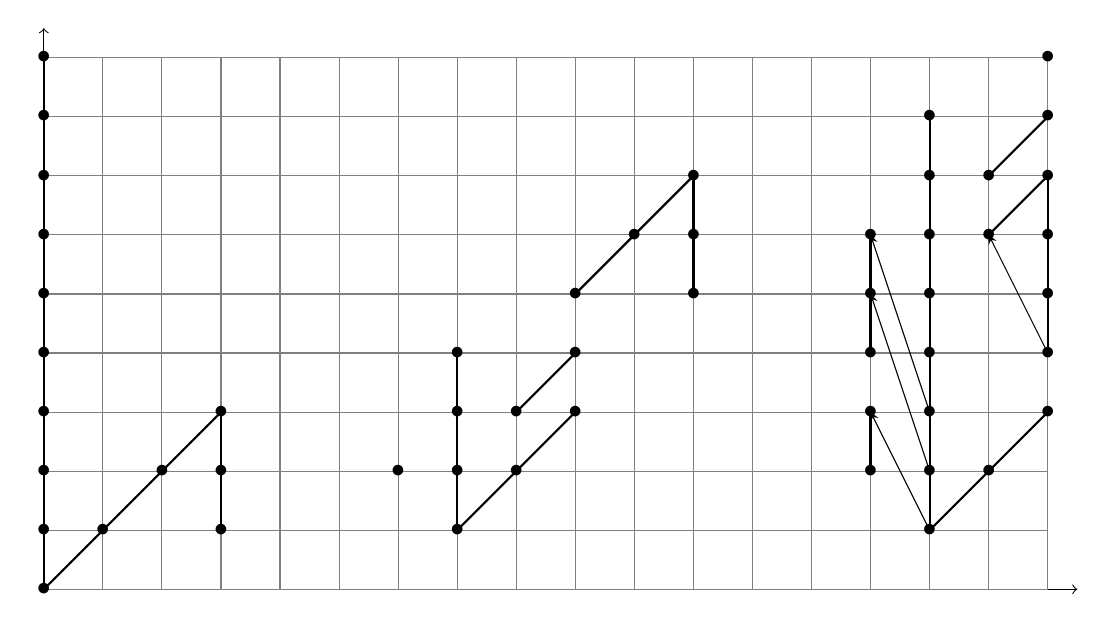
\begin{tikzpicture}[scale=0.75]
% the axes
\draw [<->] (0,9.5) |- (0,0) |- (17.5,0);
% the grid
\draw[black!50] (0,0) grid (17,9);

% the groups
\foreach \y in {0,...,9}
    {\node (one\y) at (0,\y) {$\bullet$};};
\node at (1,1) {$\bullet$};
\node at (2,2) {$\bullet$};
\node at (3,3) {$\bullet$};
\node at (3,1) {$\bullet$};
\node at (3,2) {$\bullet$};
\node at (6,2) {$\bullet$};
\node at (7,1) {$\bullet$};
\node at (7,2) {$\bullet$};
\node at (7,3) {$\bullet$};
\node at (7,4) {$\bullet$};
\node at (8,2) {$\bullet$};
\node at (8,3) {$\bullet$};
\node at (9,3) {$\bullet$};
\node at (9,4) {$\bullet$};
\node at (9,5) {$\bullet$};
\node at (10,6) {$\bullet$};
\node at (11,5) {$\bullet$};
\node at (11,6) {$\bullet$};
\node at (11,7) {$\bullet$};
\node at (14,2) {$\bullet$};
\node at (14,3) {$\bullet$};
\node at (14,4) {$\bullet$};
\node at (14,5) {$\bullet$};
\node at (14,6) {$\bullet$};
\node at (15,1) {$\bullet$};
\node at (15,2) {$\bullet$};
\node at (15,3) {$\bullet$};
\node at (15,4) {$\bullet$};
\node at (15,5) {$\bullet$};
\node at (15,6) {$\bullet$};
\node at (15,7) {$\bullet$};
\node at (15,8) {$\bullet$};
\node at (16,2) {$\bullet$};
\node at (16,6) {$\bullet$};
\node at (16,7) {$\bullet$};
\node at (17,3) {$\bullet$};
\node at (17,4) {$\bullet$};
\node at (17,5) {$\bullet$};
\node at (17,6) {$\bullet$};
\node at (17,7) {$\bullet$};
\node at (17,8) {$\bullet$};
\node at (17,9) {$\bullet$};

% multiplicative structure

\path (0,0) edge[thick] (0,9)
      (0,0) edge[thick] (3,3)
      (3,1) edge[thick] (3,3)
      (7,1) edge[thick] (7,4)
      (7,1) edge[thick] (9,3)
      (8,3) edge[thick] (9,4)
      (9,5) edge[thick] (11,7)
      (11,5) edge[thick] (11,7)
      (14,2) edge[thick] (14,3)
      (14,4) edge[thick] (14,6)
      (15,1) edge[thick] (15,8)
      (15,1) edge[thick] (17,3)
      (16,6) edge[thick] (17,7)
      (16,7) edge[thick] (17,8)
      (17,4) edge[thick] (17,7);

% differentials

\path (15,1) edge[-stealth] (14,3)
      (15,2) edge[-stealth] (14,5)
      (15,3) edge[-stealth] (14,6)
      (17,4) edge[-stealth] (16,6);
\end{tikzpicture}
\end{center}
\caption{The $H\F_2$-Adams spectral sequence for the sphere, beginning at the second page.  Thin lines denote multiplication by $2$ and by $\eta$, thin arrows denote $d_2$-- and $d_3$--differentials.}\label{HF2ASSFigure}
\end{figure}
\end{example}

\todo{Jon asked: spectral sequences coming from $\pi_*$ of a Tot tower increase Tot degree. ANSS differentials decrease degree: they run against the multiplicative structure in pictures. What's going on with this?  I think this is a duality effect: working with the Steenrod algebra versus its dual.}









\section{The unoriented bordism ring}

Our goal today is to use the results of the previous lectures to make a calculation of $\pi_* MO$, the unoriented bordism ring.  The Adams spectral sequence converging to this has signature \[H^*_{\mathrm{gp}}(\InternalAut(\G_a); \widetilde{H\F_2P_0(MO)}) \Rightarrow \pi_* MO,\] and so we see that we need to understand $H\F_2P_0(MO)$, together with its comodule structure over the dual Steenrod algebra.

Our first step toward this is the following calculation:
\begin{lemma}
$H\F_2P^0 BO(n) \cong \F_2 \llbracket w_1, \ldots, w_n \rrbracket$.
\end{lemma}
\begin{proof}
The orthogonal groups sit in coset fibration sequences \[O(n-1) \to O(n) \to S^{n-1},\] and delooping the groups gives a rotated spherical fibration \[S^{n-1} \to BO(n-1) \to BO(n).\]  The associated Serre spectral sequence shows that $H\F_2P^0 BO(n)$ must have one extra free generator in it to receive a differential from the exterior generator of $H\F_2P^0 S^{n-1}$.  Noting $BO(1) \simeq \RP^\infty$, our discussion from previous lectures takes care of the base case.
\end{proof}

\begin{corollary}
There is a triangle
\begin{center}
\begin{tikzcd}
& \Sym H\F_2P_0 BO(1) \arrow{d}{\simeq} \\
H\F_2P_0 BO(1) \arrow{r} \arrow{ru} & H\F_2P_0 BO. \qed
\end{tikzcd}
\end{center}
\end{corollary}
\noindent We will defer the proof of this until \Cref{ComplexBordismChapter}, since it requires knowing that \[H\F_2P^0 BO(k) \to H\F_2P^0 BO(1)^{\times k}\] is injective, which we will revisit later anyhow.\oweproof{$H_* BO$ is a symmetric algebra on $H_* BO(1)$}

With this in hand, however, we can uncover the ring structure on $H\F_2P_0 MO$:
\begin{corollary}\label{HF2MOisFree}
There is also a triangle
\begin{center}
\begin{tikzcd}
& \Sym H\F_2P_0 MO(1) \arrow{d}{\simeq} \\
H\F_2P_0 MO(1) \arrow{r} \arrow{ru} & H\F_2P_0 MO.
\end{tikzcd}
\end{center}
In particular, $H\F_2P_0 MO \cong \F_2[b_1, b_2, \ldots]$.
\end{corollary}
\begin{proof}
The block sum maps \[BO(n) \times BO(m) \to BO(n+m)\] Thomify to give compatible maps \[MO(n) \sm MO(m) \to MO(n+m).\]  Taking the limit in $n$ and $m$, this gives a ring structure on $MO$ compatible with that on $BO$.  The Corollary then follows from the functoriality of Thom isomorphisms.
\end{proof}

We now seek to understand the scheme $\Spec H\F_2P_0 MO$, and in particular its action of $\InternalAut(\G_a)$.  Our launching-off point for this is a topological version of the ``freeness'' result in the previous Corollary:
\begin{lemma}\label{DetectingMORingMapsInHomotopy}
The following square commutes:
\begin{center}
\begin{tikzcd}
\CatOf{Modules}_{\F_2}(H\F_2P_0 MO, \F_2) & \CatOf{Spectra}(MO, H\F_2P) \arrow{l}{\simeq} \\
\CatOf{Algebras}_{\F_2/}(H\F_2P_0 MO, \F_2) \arrow[hookrightarrow]{u} & \CatOf{RingSpectra}(MO, H\F_2P) \arrow{l}{\simeq} \arrow[hookrightarrow]{u}.
\end{tikzcd}
\end{center}
\end{lemma}
\begin{proof}
The top isomorphism is asserting only that $\F_2$--cohomology and $\F_2$--homology are linearly dual to one another.  The second follows immediately from investigating the effect of the ring homomorphism diagrams in the bottom-right corner in terms of the subset they select in the top-left.
\end{proof}

\begin{corollary}
There is a correspondence between homotopy classes of ring maps $MO \to H\F_2P$ and homotopy classes of factorizations
\begin{center}
\begin{tikzcd}
\S^0 \arrow{r} & MO(1) \arrow[densely dotted]{d} \\
& H\F_2P.
\end{tikzcd}
\end{center}
\end{corollary}
\begin{proof}
Given a ring map $MO \to H\F_2P$, we can restrict it along the inclusion $MO(1) \to MO$ to produce a particular cohomology class \[f \in H\F_2P^0 MO(1) = \CatOf{Modules}_{\F_2}(H\F_2P_0 MO(1), \F_2).\]  Interpreting $f$ as such a function, it is determined by its behavior on the basis of vectors in $\widetilde{H\F_2P}_0 MO(1)$ dual to the powers of the usual coordinate $x \in H\F_2^1 \RP^\infty$.  Finally, given \emph{any} module map $\widetilde{H\F_2P}_0 MO(1) \to \F_2$, we can employ \Cref{HF2MOisFree} and to produce an algebra map $H\F_2P_0 MO \to \F_2$ and hence \Cref{DetectingMORingMapsInHomotopy} gives a ring spectrum map $MO \to H\F_2P$.
\end{proof}

\begin{corollary}
There is an $\InternalAut(\G_a)$--equivariant isomorphism of schemes between $\Spec H\F_2P_0 MO$ and $\Coord_1(\RP^\infty_{H\F_2P})$, the scheme of coordinate functions on $\RP^\infty_{H\F_2P} \to \A^1$ which restrict to the canonical identification of tangent spaces $\RP^1_{H\F_2P} = \A^{1,(1)}$.
\end{corollary}
\begin{proof}
The method of the previous proof is to exhibit a isomorphism between these schemes.  To learn that this isomorphism is equivariant for $\InternalAut(\G_a)$, you need only know that the image of the map $BO(1) \to BO$ on mod--$2$ homology generates $H\F_2P_0 BO$ as an algebra.\todo{This is clumsily stated.}
\end{proof}

We are now ready to analyze the group cohomology of $\InternalAut(\G_a)$ with coefficients in the comodule $H\F_2P_0 MO$.
\begin{theorem}
The action of $\InternalAut_1(\G_a)$ on $\Coord_1(\G_a)$ is free, where $\InternalAut_1(\G_a)$ is defined by the kernel sequence \[0 \to \InternalAut_1(\G_a) \to \InternalAut(\G_a) \to \Gm \to 0.\]
\end{theorem}
\begin{proof}
Consider a point $f \in \Coord_1(\G_a)(R)$, which in terms of the standard coordinate can be expressed as \[f(x) = \sum_{j=1}^\infty b_{j-1} x^j,\] where $b_0 = 1$.  Decompose this series as $f(x) = f_2(x) + f_r(x)$, with
\begin{align*}
f_2(x) & = \sum_{k=0}^\infty b_{2^k-1} x^{2^k}, &
f_r(x) & = \sum_{j \ne 2^k} b_{j-1} x^j.
\end{align*}
Note that $f_2$ gives a point $f_2 \in \InternalAut_1(\G_a)(R)$, so we can de-scale by it to give a new coordinate $g(x) = f_2^{-1}(f(x))$ with analogous series $g_2(x)$ and $g_r(x)$.  Note that $g_2(x) = x$ and that $f_2$ is the unique point in $\InternalAut_1(\G_a)(R)$ that has this property.
\end{proof}

\begin{corollary}
$\pi_* MO = \F_2[b_j \mid j \ne 2^k - 1, j \ge 1]$ with $|b_j| = j$.
\end{corollary}
\begin{proof}
Set $M = \F_2[b_j \mid j \ne 2^k - 1]$.  \todo{Compare this with the base change theorems from the previous day.} It follows from the above that the $\InternalAut_1(\G_a)$--cohomology of $H\F_2P_0(MO)$ has amplitude $0$:\todo{Maybe you should justify the step that looks like reassociation of the tensor and cotensor products. You almost definitely proved this on the previous day.}
\begin{align*}
\Cotor_{\mathcal A_*}^{*, *}(\F_2, H\F_2P_0(MO)) & = \Cotor_{\mathcal A_*}^{*, *}(\F_2, \mathcal A_* \otimes_{\F_2} M) \\
& = \F_2 \cotensor_{\mathcal A_*} (\mathcal A_* \otimes_{\F_2} M) \\
& = \F_2 \otimes_{\F_2} M = M.
\end{align*}
Since the Adams spectral sequence \[H^*_{\mathrm{gp}}(\InternalAut_1(\G_a); H\F_2P_0(MO)) \Rightarrow \pi_* MO\] is concentrated on the $0$--line, it collapses.  Using the residual $\Gm$--action to infer the grading, we thus deduce \[\pi_* MO = \F_2[b_j \mid j \ne 2^k-1]. \qedhere\]
\end{proof}

This is pretty remarkable: some big statement about manifold geometry came down to understanding how we could reparametrize a certain formal group, itself a (fairly simple) purely algebraic problem.  We could close here, but there's an easy homotopical consequence of this fact that is worth recording before we leave:

\begin{lemma}
$MO$ splits as a wedge of shifts of $H\F_2$.
\end{lemma}
\begin{proof}
We have a $\pi_*$--injection $MO \to H\F_2 \sm MO$.  Pick an $\F_2$--basis $\{v_\alpha\}_\alpha$ for $\pi_* MO$ and extend it to a $\F_2$--basis $\{v_\alpha\}_\alpha \cup \{w_\beta\}_\beta$ for $H\F_2 \sm MO$.  Altogether, this larger basis can be represented as a single map \[\bigvee_\alpha \Susp^{m_\alpha} \S \vee \bigvee_\beta \Susp^{n_\beta} \S \xrightarrow{\bigvee_\alpha v_\alpha \vee \bigvee_\beta w_\beta} H\F_2 \sm MO.\]  Smashing through with $H\F_2$ gives an equivalence \[\bigvee_\alpha \Susp^{m_\alpha} H\F_2 \vee \bigvee_\beta \Susp^{n_\beta} H\F_2 \xrightarrow\simeq H\F_2 \sm MO.\]  The composite map \[MO \to H\F_2 \sm MO \xleftarrow\simeq \bigvee_\alpha \Susp^{m_\alpha} H\F_2 \vee \bigvee_\beta \Susp^{n_\beta} H\F_2 \to \bigvee_\alpha \Susp^{m_\alpha} H\F_2\] is a weak equivalence.
\end{proof}

\begin{remark}
Just using that $\pi_* MO$ is connective and $\pi_0 MO = \F_2$, we can produce a ring spectrum map $MO \to H\F_2$.  What we've learned is that this map has a splitting: $MO$ is also an $H\F_2$--algebra.
\end{remark}

\todo[inline]{Should you eventually mention the stable cooperations $MO^{MO}$?  Rather than coming with a specified logarithm, it's an isomorphism between any pair of additive formal groups --- or, I suppose, a pair of logarithms.}


